\chapter{Аналитическая часть}
\section{Анализ предметной области}
Предметной областью данной работы является сегмент предприятий общественного питания, специализирующихся на реализации напитков -- кофейни.

Основные компоненты предметной области включают:
\begin{itemize}
	\item сетевые структуры кофеен, состоящие из одного или более заведений;
	\item кофейни, относящиеся к определенной сети;
	\item напитки, которые включает в себя меню заведений;
	\item меню, в котором для покупателей указываются цены и размеры напитков;
	\item программы лояльности, помогающие кофейням удерживать и привлекать клиентов за счет, например, различных акций и скидок на напитки.
\end{itemize}

\section{Анализ существующих решений}
Существует достаточно большое количество приложений, предоставляющих пользователям возможность просмотра информации о кофейнях и поиска среди них подходящего заведения. Наиболее известными являются:
\begin{itemize}
\item Кофейная карта~\cite{coffee_kart};
\item Coffee Forest~\cite{coffee_forest};
\item Яндекс Карты~\cite{yandex}.
\end{itemize}

Для сравнения существующих решений были выделены следующие критерии:
\begin{itemize}
	\item возможность просмотра информации о кофейнях в приложении;
	\item возможность просмотра меню кофеен в приложении;
	\item возможность составления списка избранных кофеен;
	\item возможность составления списка избранных напитков;
	\item возможность поиска кофеен на основе наличия в их меню определенного напитка.
\end{itemize}

В таблице~\ref{pop_apps} представлены результаты сравнения упомянутых ранее приложений по выделенным критериям.

\newpage
\begin{table}[ht]
	\begin{center}
		\begin{threeparttable}
			\caption{\label{pop_apps} Сравнение существующих решений}
			\begin{tabular}{|p{6cm}|p{3cm}|p{2cm}|p{2cm}|c|}
				\hline
				\textbf{Критерий сравнения} & \textbf{Кофейная карта} & \textbf{Coffee Forest} & \textbf{Яндекс Карты} \\ \hline
				Возможность просмотра информации о кофейнях в приложении & Да & Да & Да \\ \hline
				Возможность составления списка избранных кофеен & Да & Да & Да \\ \hline
				Возможность просмотра меню кофеен в приложении  & Нет & Нет & Да \\ \hline
				Возможность составления списка избранных напитков & Нет & Нет & Нет \\ \hline
				Возможность поиска кофеен на основе наличия в их меню определенного напитка & Нет & Нет & Нет \\ \hline
			\end{tabular}
		\end{threeparttable}
	\end{center}
\end{table}

Таким образом, вышеперечисленные приложения не предоставляют пользователям возможностей создания списка избранных напитков и поиска кофеен на основе наличия в их меню определенного напитка.

\section{Анализ существующих моделей баз данных}
База данных -- это самодокументированное собрание интегрированных записей. База данных хранит сведения о предметной области, используемые в прикладных системах для удовлетворения информационных потребностей пользователя~\cite{struzhkin}.


Разработка базы данных всегда сопровождается моделью данных, которая позволяет наглядно представить структуру хранимых данных и связи между ними. Выделяют 3 основных типа моделей организации данных:

\begin{itemize}
	\item дореляционная модель;
	\item реляционная модель;
	\item постреляционная модель.
\end{itemize}

\subsection{Дореляционная модель}
Дореляционная модель организации данных разделяется на:
\begin{itemize}
	\item иерархическую;
	\item сетевую.
	
\end{itemize}

\textbf{Иерархическая} модель данных представляется набором деревьев, связанных друг с другом по принципу построения иерархических структур~\cite{struzhkin}. Связи между записями выражаются в виде отношений предок/потомок, при чем у каждой записи есть ровно одна родительская запись. При этом если удаляется родительская запись, то автоматически должны быть удалены все дочерние записи. Это помогает поддерживать ссылочную целостность. В иерархической модели реализуется только связь типа 1:N (<<один--ко--многим>>), при чем только в направлении от родительского элемента к дочернему. На рисунке~\ref{hierarchy} представлена общая схема иерархической модели.

\begin{figure}[H]
	\centering
	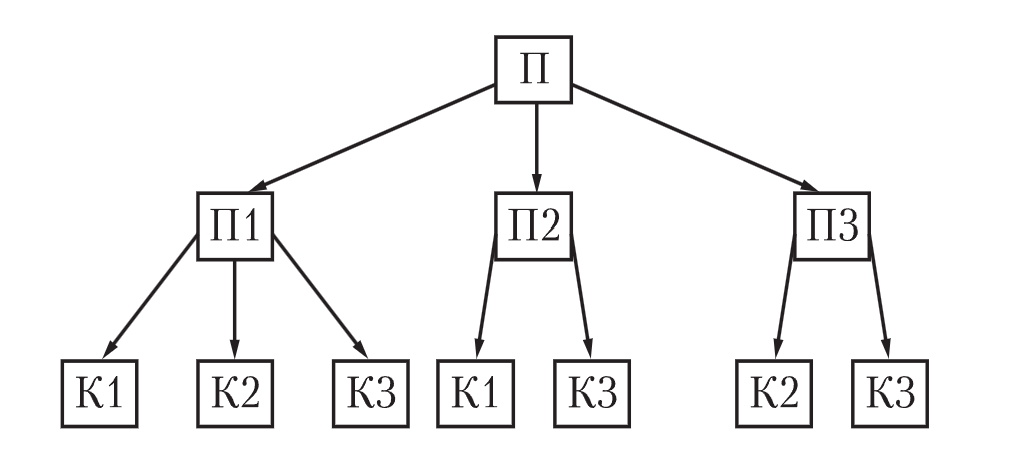
\includegraphics[width=0.6\linewidth]{img/hierarchy.png}
	\caption{Общая схема иерархической модели данных}
	\label{hierarchy}
\end{figure}

\textbf{Сетевая} модель данных является расширением иерархической модели. Сетевая модель позволяет описывать связи M:N (<<многие--ко--многим>>), чтобы одна запись могла участвовать в нескольких отношениях предок/потомок. Сетевые базы данных могут быть представлены в виде графа. Для данной модели характерна высокая сложность организации структуры памяти и жесткость модели, что приводит к необходимости полного  пересмотра модели при появлении новых условий в предметной области, требующих внесения изменений в структуру данных~\cite{struzhkin}. На рисунке~\ref{network} представлена структура сетевой модели организации данных.


\begin{figure}[H]
	\centering
	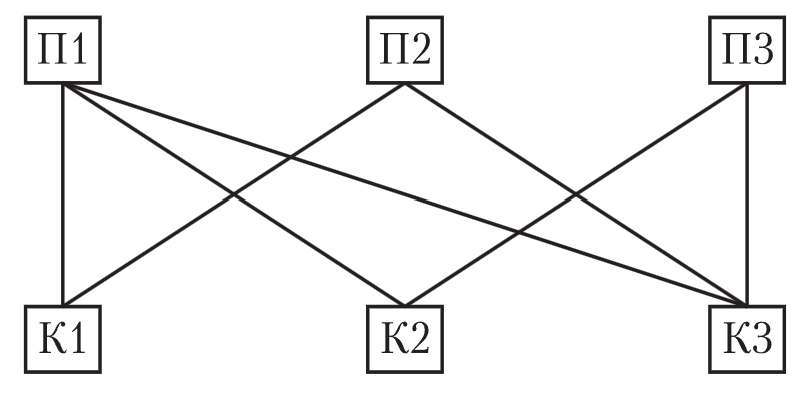
\includegraphics[width=0.5\linewidth]{img/network_db.png}
	\caption{Структура сетевой модели данных}
	\label{network}
\end{figure}

\textbf{Достоинством} дореляционной модели данных является скорость доступа к данным~\cite{ilushechkinz}.

К \textbf{недостаткам} дореляционной модели можно отнести необходимость значительных ресурсов дисковой и основной памяти компьютера, поскольку каждый элемент данных должен содержать ссылки на некоторые другие элементы~\cite{ilushechkinz}. Трудоемкость процесса изменения структуры данных и перегруженность логики деталями организации доступа к базе данных также являются недостатками этой модели.



\subsection{Реляционная модель данных}
В реляционной модели все данные и связи между ними хранятся в таблицах, а для определения структуры данных и манипулирования их значениями используют язык SQL (Structured Query Language -- структурированный язык запросов). Реляционная модель опирается на систему понятий, важнейшими из которых являются тип данных, домен, атрибут, кортеж, первичный и внешний ключ.  


Домен -- допустимое потенциальное множество значений какого-то
типа данных. 

Атрибут отношения -- это пара вида <имя\textunderscore атрибута, имя\textunderscore домена>. Атрибут является некоторой характеристикой сущности.

Схемой отношения называется именованное множество упорядоченных пар <имя\textunderscore атрибута, имя\textunderscore домена>. 

Кортеж -- это множество упорядоченных пар вида <имя\textunderscore атрибута, значение\textunderscore атрибута>, которое содержит одно вхождение каждого имени атрибута, принадлежащего схеме отношения.

Отношение, определенное на множестве из n доменов (не обязательно различных), содержит две части: заголовок (схему отношения) и тело (множество из m кортежей).

Атрибут, значение которого идентифицирует кортеж, называется ключом отношения. Среди всех ключей выбирается один первичный, который должен быть уникальным и неизбыточным. Для организации взаимосвязи отношений используется внешний ключ.


\textbf{Реляционная база данных} -- это набор отношений, имена которых совпадают с именами схем отношений в схеме базы данных. На рисунке~\ref{relyac_example} представлен пример отношения (таблицы) реляционной базы данных.

\begin{figure}[H]
	\centering
	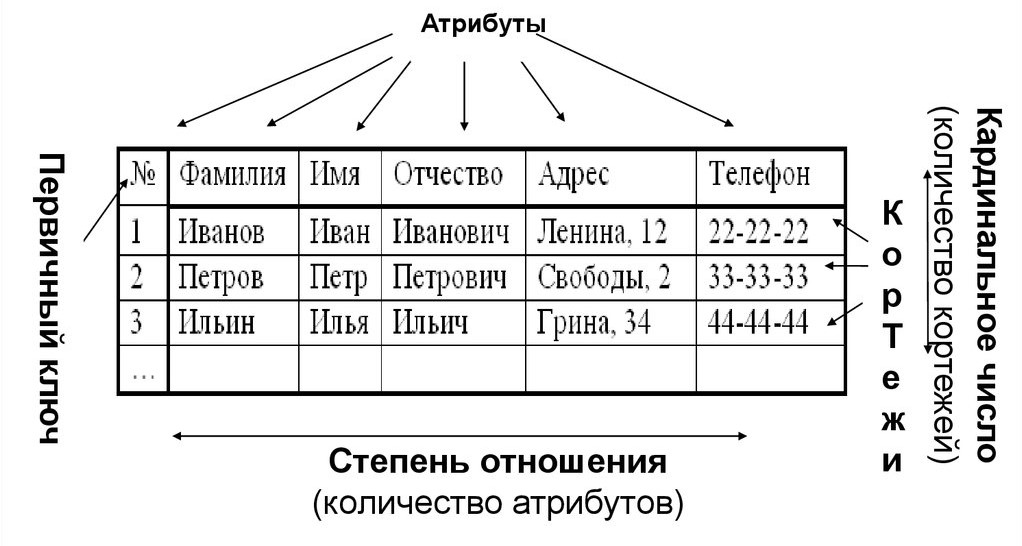
\includegraphics[width=0.8\linewidth]{img/relyac_db.jpg}
	\caption{Пример таблицы реляционной базы данных}
	\label{relyac_example}
\end{figure}

\textbf{Преимуществами} реляционной модели являются согласованность данных, сравнительная простота инструментальных средств ее поддержки~\cite{ilushechkinz}, независимость прикладных программ от правил хранения и размещения сведений в базе данных~\cite{struzhkin}.

К \textbf{недостаткам} реляционной модели относят зависимость скорости выполнения операций от размера таблиц~\cite{ilushechkinz}, ограничение в структурах представления данных, так как все данные хранятся в виде отношений, состоящих из простых атрибутов~\cite{markin}.

\subsection{Постреляционные базы данных}
Постреляционная модель организации данных представляет собой развитие реляционного подхода. Ее основной целью является расширение возможностей баз данных в тех областях, где реляционная модель и SQL недостаточно гибки~\cite{markin}.

Постреляционная модель снимает ограничение неделимости данных, допуская многозначные поля, и не накладывает требования на длину и количество полей в записях, что делает структуру таблиц более гибкой и наглядной.

К \textbf{достоинствам} постреляционной модели относят возможность работы со сложными и неструктурированными данными, а также большими объемами информации и большим количеством пользователей.

\textbf{Недостатком} постреляционной модели является сложность обеспечения целостности и непротиворечивости данных, хранимых в ней~\cite{markin}.


\section{Выбор модели хранения данных}
В качестве модели организации данных, которая будет использована в курсовой работе, была выбрана реляционная модель, поскольку она позволяет обеспечить структурированное хранение данных и их целостность.

\section{Формализация задачи}
Необходимо разработать базу данных, которая будет хранить информацию о кофейнях и их меню напитков, а также приложение для доступа к ней. Приложение должно предоставлять пользователям возможность регистрации и авторизации, просмотра информации о сетях кофеен, их меню и открытых филиалах, поиска кофеен, в которых продается определенный напиток. Также приложение должно позволять составлять список избранных напитков и список избранных кофеен. Реализовать возможность четырех уровней доступа: для гостей (неавторизованных пользователей), обычных пользователей (авторизованных), модераторов и администраторов.




\subsection{Типы пользователей}

Пользователи проектируемого приложения делятся на 4 типа:
\begin{itemize}
	\item неавторизованный пользователь (гость);
	\item авторизованный пользователь;
	\item модератор;
	\item администратор.
\end{itemize} 

В таблице~\ref{users_descr} представлено описание типов пользователей проектируемого приложения.

\begin{table}[ht]
	\begin{center}
		\begin{threeparttable}
			\caption{\label{users_descr} Описание типов пользователей приложения}
			\begin{tabular}{|p{6cm}|p{10cm}|c|}
				\hline
				
				
				\textbf{Тип пользователя} & \textbf{Возможности}  \\ \hline
				Неавторизованный пользователь (Гость) & Регистрация,  авторизация.\\ \hline
				Авторизованный пользователь & Просмотр информации о сетях кофеен, напитках, кофейнях и программах лояльности сетей кофеен, составление списка избранных напитков и кофеен, а также поиск сети, в меню которой есть выбранный пользователем напиток, изменение данных профиля и удаление аккаунта . \\ \hline
				Модератор & Все возможности авторизованного пользователя, а также добавление и удаление записей таблицы меню, таблицы напитков, таблицы кофеен.\\ \hline
				Администратор & Все возможности модератора, а также просмотр списка пользователей, изменение прав доступа пользователей и удаление их аккаунтов.\\ \hline
				
			\end{tabular}
		\end{threeparttable}
	\end{center}
\end{table}



На рисункe~\ref{usecase_all} представлена диаграмма прецедентов.

\begin{figure}[H]
	\centering
	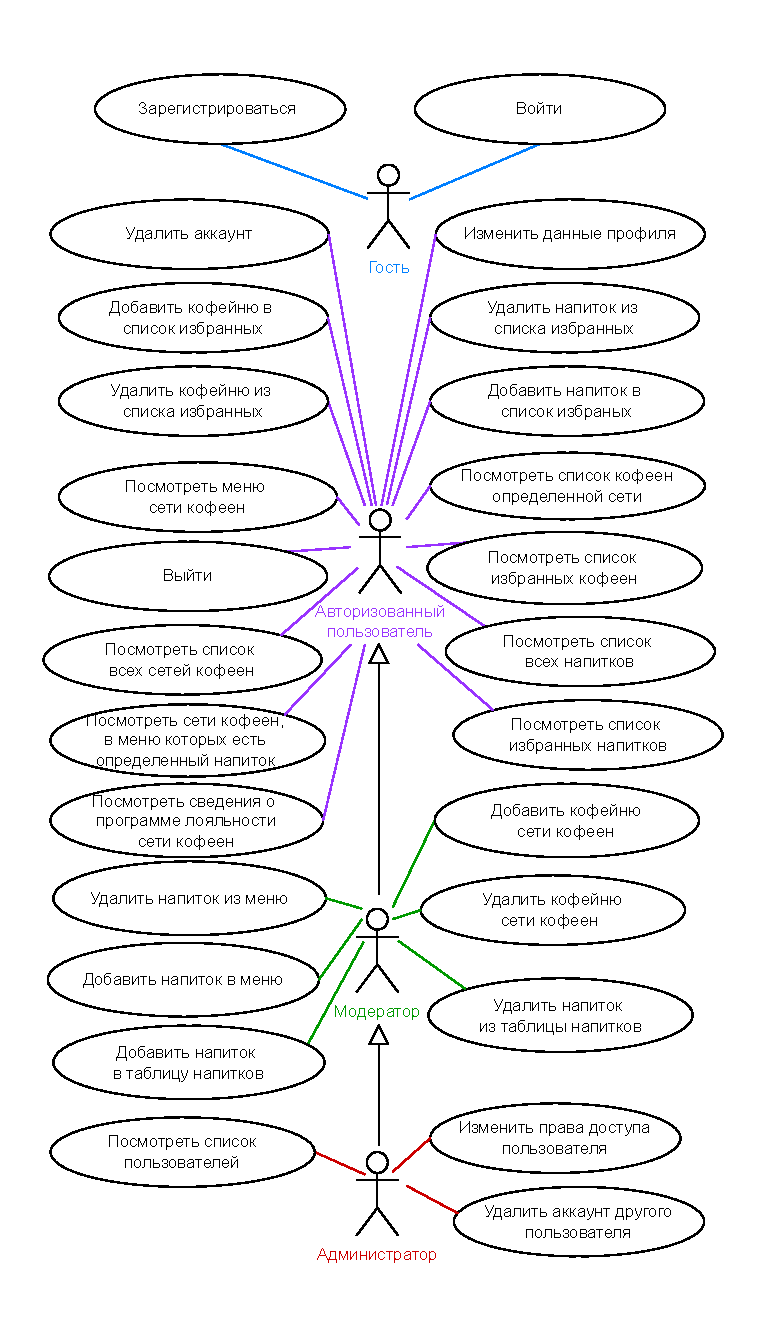
\includegraphics[width=0.8\linewidth]{img/usecase2605.pdf}
	\caption{Диаграмма прецедентов}
	\label{usecase_all}
\end{figure}
\newpage



\subsection{Формализация данных}
Согласно поставленной задаче, база данных должна содержать сущности, описанные в таблице~\ref{er_descr}.

\begin{table}[ht]
	\begin{center}
		\begin{threeparttable}
			\caption{\label{er_descr} Описание сущностей базы данных}
			\begin{tabular}{|p{6cm}|p{10cm}|c|}
				\hline
				\textbf{Сущность} & \textbf{Описание}  \\ \hline
				Пользователь & Id, логин, пароль, дата рождения, почта, Id роли\\ \hline
				Роль & Id, название\\ \hline
				Сеть кофеен & Id, название, сайт, количество кофеен\\ \hline
				Кофейня & Id, Id сети кофеен, адрес, часы работы\\ \hline
				Программа лояльности & Id, Id сети кофеен, тип, описание\\ \hline
				Напиток & Id, название\\ \hline
				Категория напитка & Id, название\\ \hline
			\end{tabular}
		\end{threeparttable}
	\end{center}
\end{table}

На рисунке~\ref{er_img} представлена диаграмма сущность-связь базы данных.


\begin{figure}[H]
	\centering
	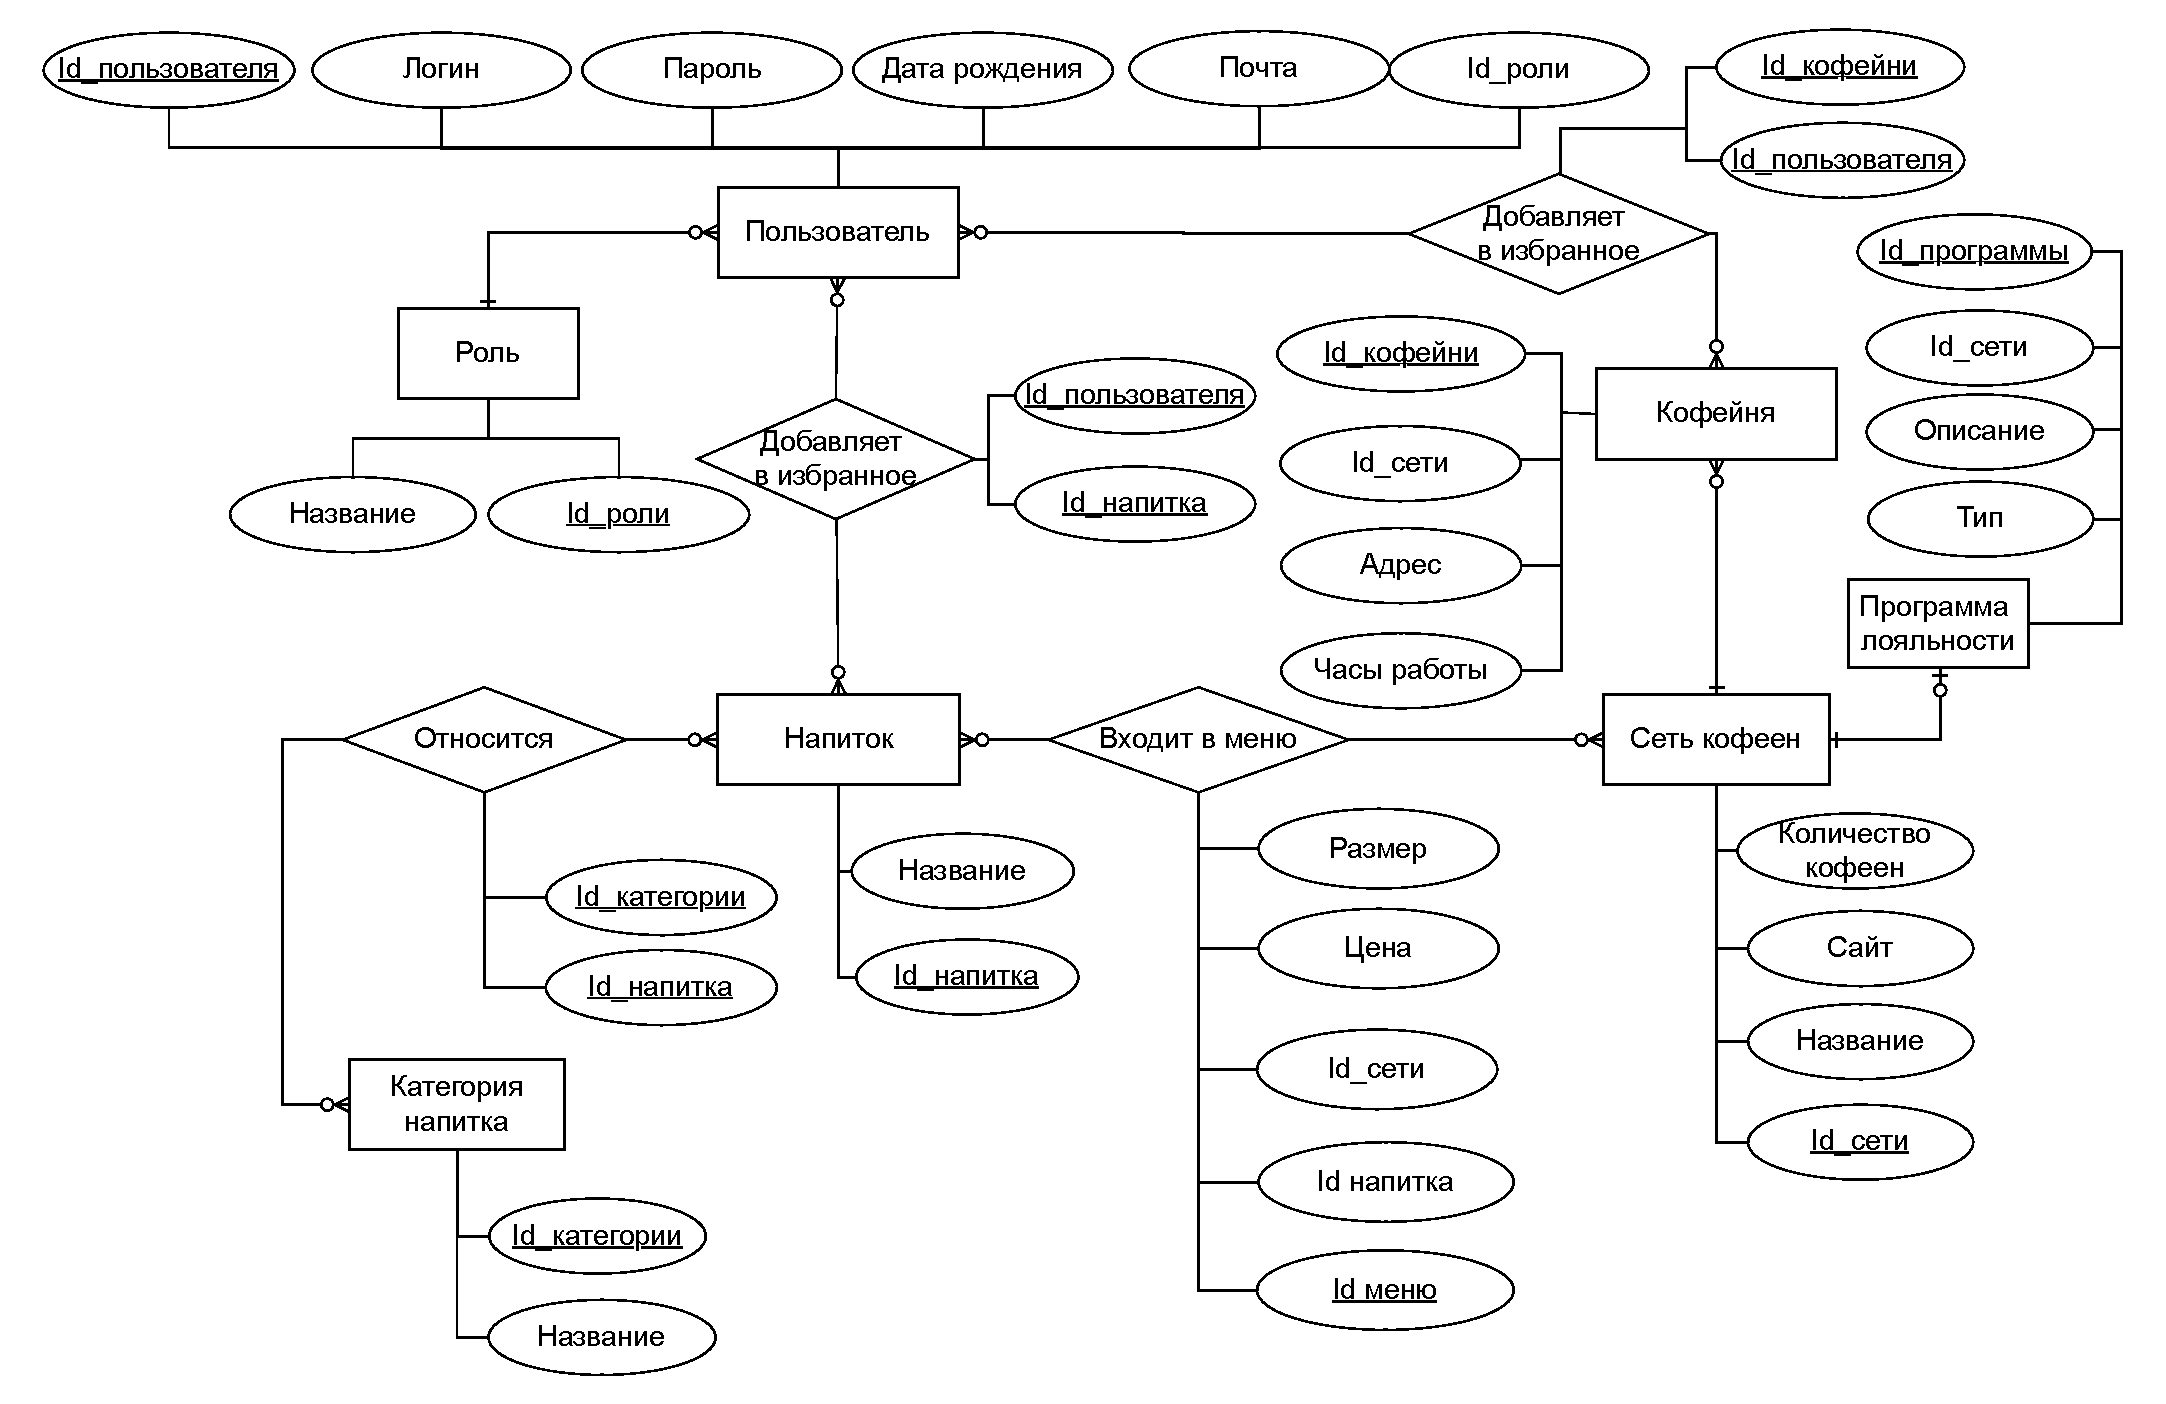
\includegraphics[width=1\linewidth]{img/er_last.pdf}
	\caption{Диаграмма сущность-связь базы данных}
	\label{er_img}
\end{figure}


\section*{Вывод}
В данной части был проведен анализ предметной области, существующих решений и моделей баз данных, описаны типы пользователей проектируемого приложения и данные, хранящиеся в базе данных. В качестве модели организации данных была выбрана реляционная модель.


